\documentclass[12pt]{book}

% Paquetes comunes
% common/preamble.tex — paquetes y configuración compartida
\usepackage[utf8]{inputenc}
\usepackage[T1]{fontenc}
\usepackage{lmodern}
\usepackage{geometry}
\usepackage{graphicx}
\usepackage{xcolor}
\usepackage{hyperref}
\usepackage{parskip}
\usepackage{amsmath, amssymb}

\geometry{margin=2.5cm}
\hypersetup{
    colorlinks=true,
    linkcolor=blue,
    urlcolor=blue,
    citecolor=blue
}


% Rutas de figuras de este módulo
\graphicspath{{figures/}}

\title{Libro de Ejemplo — Módulo 1}
\author{Autor del Diplomado}
\date{\today}

\begin{document}
\frontmatter
\maketitle

\tableofcontents

\mainmatter

\chapter{Introducción}
Este es un \textbf{monorepo} de ejemplo con un libro y un formato tipo Cornell.
Compila con \texttt{latexmk} y genera artefactos en \texttt{latex.out/}.

\section{Figura de ejemplo}
La Figura~\ref{fig:plot} se incluye desde \texttt{figures/ejemplo\_plot.png}.

\begin{figure}[h]
    \centering
    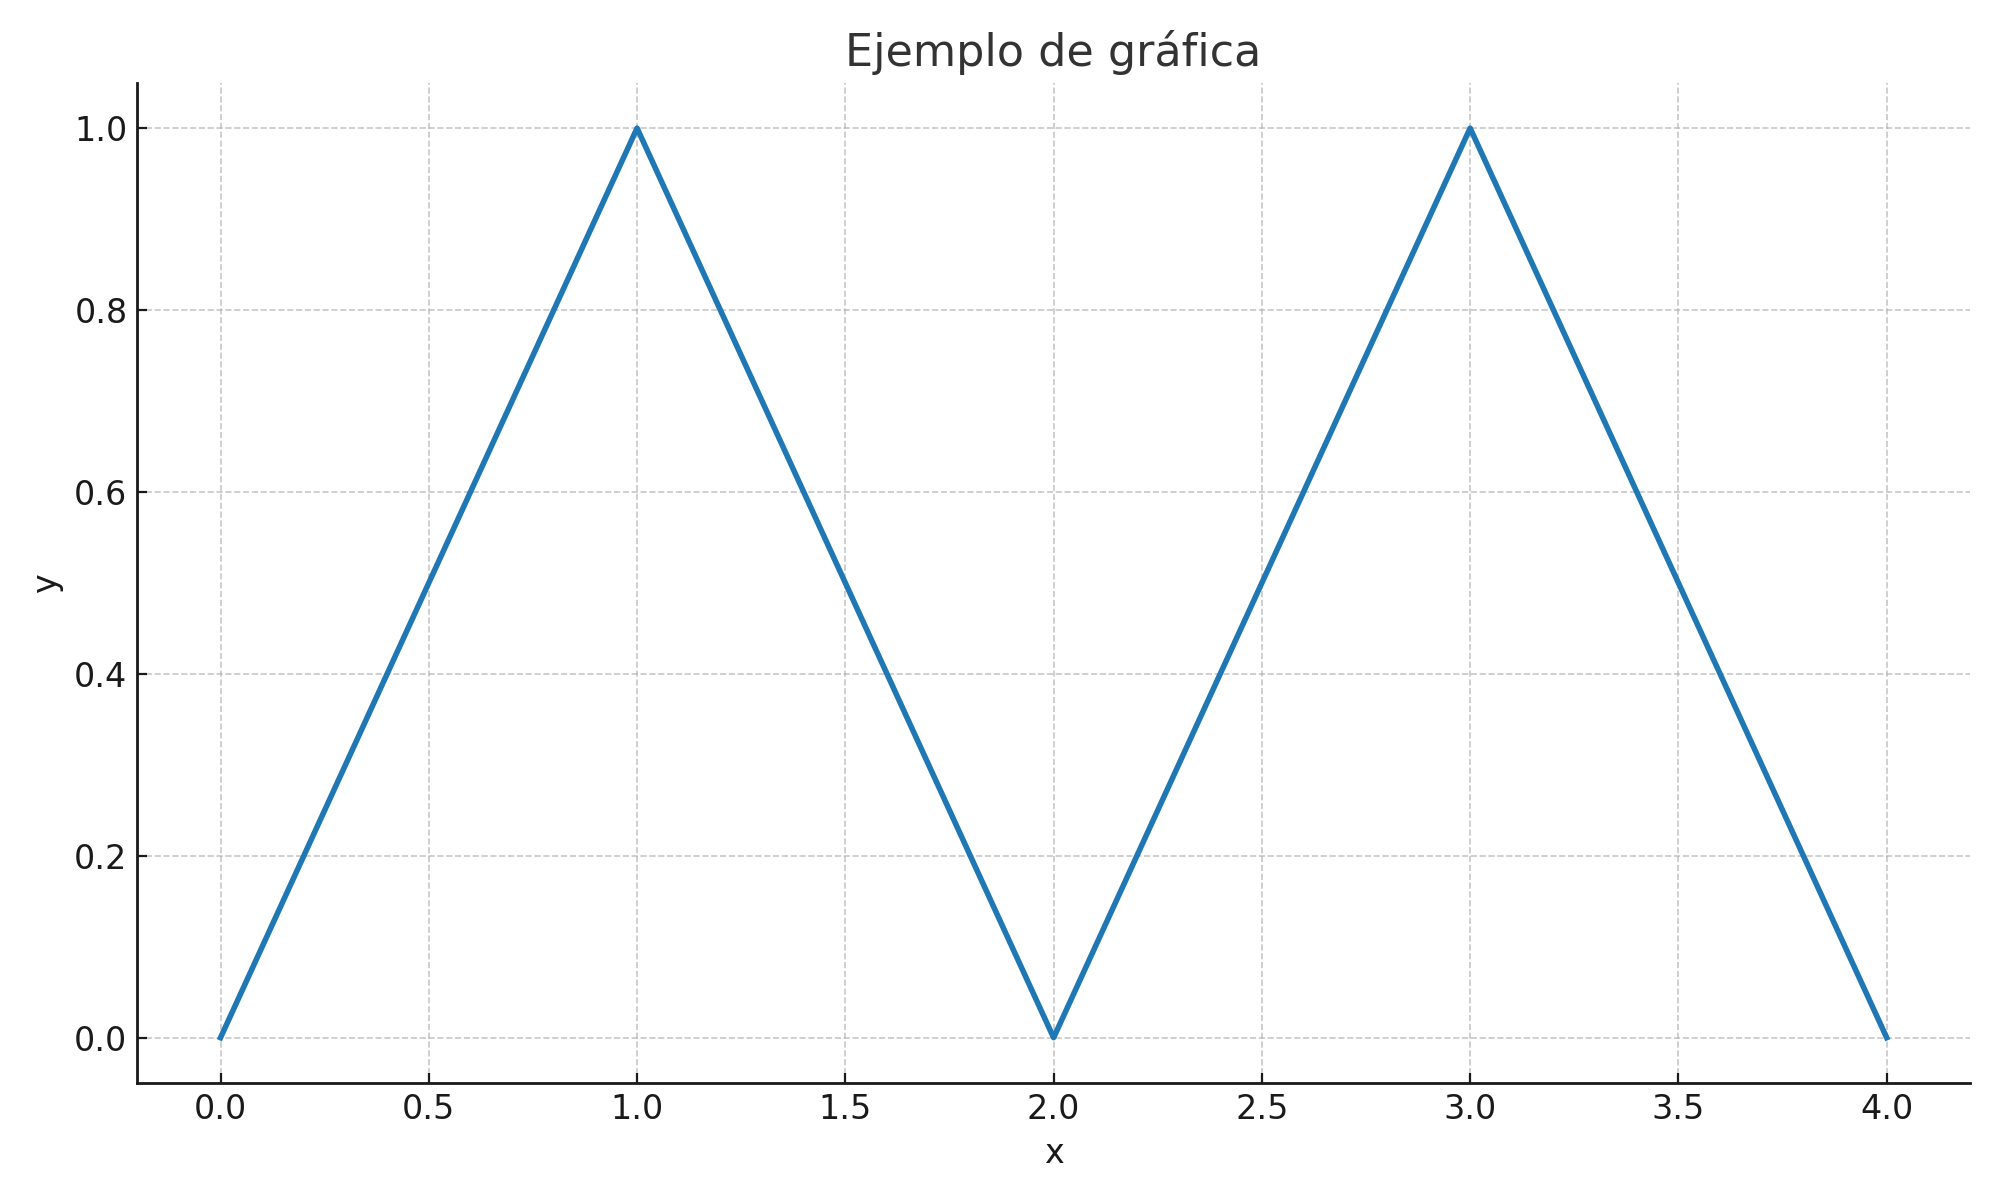
\includegraphics[width=0.7\linewidth]{ejemplo_plot.png}
    \caption{Gráfica de ejemplo generada automáticamente.}
    \label{fig:plot}
\end{figure}

\chapter{Contenido separado}
\begin{titlepage}
\newgeometry{left=7.5cm} %defines the geometry for the titlepage
\pagecolor{titlepagecolor}
\noindent
{\Huge{\textcolor{white}{Diplomado Ciencia de Datos con Python}}} \\[-1em]

\begin{figure}[h]
    \centering
    
\includegraphics[width=0.7\linewidth]{logo.png}
\end{figure}

\color{white}
\makebox[0pt][l]{\rule{1.3\textwidth}{1pt}}
\par
\noindent
%\textbf{\textsf{Diplomado Ciencia de Datos con Python}} %\textcolor{namecolor}{\textsf{Ingenier\'ia}}
\vfill
\noindent
{\huge \textsf{Módulo 1, Versión 0.0.1}}
\vskip\baselineskip
\noindent
\textsf{\today}
\end{titlepage}
\restoregeometry % restores the geometry
\nopagecolor% Use this to restore the color pages to white
%
\section*{Dedicatoria}
A quienes disfrutan de \LaTeX{}, el versionado limpio y los documentos reproducibles.

\section*{Autoría}
Autor: Nombre del autor.\\
Contacto: autor@correo.com


\chapter{Introducción}
El propósito de este tema es introducirte en el mundo de la programación de computadoras
usando el lenguaje de Python. Aprenderás lo indispensable para el desarrollo de software,
se te mostrare el objetivo del lenguaje, su historia y las herramientas necesarias para dar el
salto al mundo de desarrollo

\section{Lenguaje de Programación Python.}

Antes de comenzar a desarrollar de lleno, tienes que saber lo que es Python y la
importancia de aprenderlo.

\textbf{¿Qué es Python?}\\

Python es un lenguaje de programación interpretado, multiparadigma. Sus estructuras de
datos integradas de alto nivel, combinadas con tipado y enlace dinámicos, lo hacen muy
atractivo para el desarrollo rápido de aplicaciones, así como para su uso como lenguaje de
scripts.

\textbf{¿Por qué la gente usa Python?}\\

Dentro del mundo del desarrollo existen muchos lenguajes de programación en la
actualidad, esta pregunta es de las más concurridas. Python es uno de los lenguajes de
programación con más usuarios con forme al tiempo. En una encuesta dentro de los
lenguajes más reconocidos se encuentra Python de acuerdo a Tiobe Ranking. (TIOBE
Software BV, 2021)

De acuerdo con la gráfica podemos notar que se encuentra entre los primeros tres, esto nos
permite demostrar que durante el tiempo la comunidad va creciendo cada vez más.
Algunas de las razones por las que se utiliza Python parecen ser estos:
Software de calidad.
Para muchos, el enfoque de Python es la legibilidad, la coherencia y la calidad del software,
estos puntos en general lo distinguen entre otras herramientas en el mundo de las
secuencias de comandos. El código Python está diseñado para ser legible y, por lo tanto,
reutilizable y mantenible, mucho más que los tradicionales lenguajes de secuencias de
comandos. La uniformidad del código Python hace que sea fácil de entender.
Productividad del desarrollador
Python aumenta la productividad del desarrollador muchas veces más allá de compilado o
estáticamente lenguajes mecanografiados como C, C ++ y Java. El código Python suele ser
de un tercio a un quinto del tamaño del código C ++ o Java equivalente. Eso significa que
hay menos para escribir, menos para depurar y menos para mantener. Los programas de
Python también se ejecutan inmediatamente, sin los largos pasos de compilación y enlace
requeridos por otras herramientas, aumentando aún más la velocidad del programador.
Portabilidad del programa
La mayoría de los programas de Python se ejecutan sin cambios en las principales
plataformas informáticas. Portabilidad El código Python entre Linux y Windows, por
ejemplo, suele ser solo una cuestión de copiar el código de un script entre máquinas.
Además, Python ofrece múltiples opciones para codificar como, por ejemplo: interfaces
gráficas de usuario de portátiles, programas de acceso a bases de datos, sistemas basados en
web y más.

Bibliotecas de apoyo
Python viene con una gran colección de funcionalidades portátiles y prediseñadas,
conocidas como biblioteca estándar. Esta biblioteca admite una variedad de tareas de
programación a nivel de aplicación, desde la coincidencia de patrones de texto hasta la
creación de scripts en red. Además, Python se puede ampliar con bibliotecas de cosecha
propia y una vasta colección de software de soporte de aplicaciones de terceros. El dominio
de terceros de Python ofrece herramientas
para la construcción de sitios web, programación numérica, acceso a puerto serie,
desarrollo de juegos y mucho más (consulte más adelante para ver una muestra).
La extensión NumPy, para ejemplo, se ha descrito como un equivalente gratuito y más
poderoso al Matlab sistema de programación numérica.
Integración de componentes
Los scripts de Python pueden comunicarse fácilmente con otras partes de una aplicación,
usando una variedad de mecanismos de integración. Estas integraciones permiten que
Python se utilice como herramienta de personalización y extensión de productos. Hoy, el
código Python se pueden llamar desde programas C y C ++, se pueden integrar con Java y
NET.
Disfrute
Debido a la facilidad de uso de Python y al conjunto de herramientas incorporado, puede
hacer que el acto de programar sea más placentero que una tarea ardua.
Aunque esto puede ser un beneficio intangible, su efecto sobre la productividad es un
activo importante. De estos factores, los dos primeros (calidad y productividad) son
probablemente los beneficios más importantes para la mayoría de los usuarios de Python y
merecen una descripción más completa.

¿Qué sectores usan Python?
Todos los lenguajes de programación no son exclusivos de un sector o un nicho, las
aplicaciones dependen más bien del conocimiento de negocio que quieres vaciar en tu
desarrollo, es cierto que para ello muchas veces necesitas de librerías con funcionalidades
para ciertas necesidades con el fin de ahorrar tiempos de desarrollo, aquí es donde entra la
fortaleza de Python.
Actualmente al contar con una comunidad muy grande y activa, se generan paquetes de
funcionalidades de todo tipo. Desde paquetes estadísticos, inteligencia artificial, desarrollo
de video juegos, etc. (Python, 2021)
Para poder encontrar la historia de éxito, dominios de aplicación y citas de usuarios de
Python puedes revisar los siguientes enlaces:

Historias de éxito: http://www.python.org/about/success
Dominios de la aplicación: http://www.python.org/about/apps
Citas de usuario: http://www.python.org/about/quotes
Hoy en día es que Python se usa en todo el mapa, en términos de dominios de aplicación.
Su propósito general lo hace aplicable a casi todos los campos, no solo a uno. De hecho, es
seguro decir que Prácticamente todos los programas de escritura de organizaciones
importantes utilizan Python, ya sea para tareas tácticas a corto plazo, como pruebas y
administración, o para estrategias a largo plazo.
Comparación de Python con otros lenguajes
Python a menudo se compara con otros lenguajes interpretados como Java, JavaScript, Perl,
Tcl o Smalltalk. En esta sección se compara brevemente Python con algunos de estos
lenguajes. Estas comparaciones se concentran únicamente en cuestiones de lenguaje. En la
práctica, la elección de un lenguaje de programación a menudo está dictada por otras
limitaciones del mundo real, como el costo, la disponibilidad, la capacitación y la inversión

previa, o incluso el vínculo emocional. Dado que estos aspectos son muy variables, parece
una pérdida de tiempo considerarlos mucho para esta comparación.
Java
Por lo general, se espera que los programas Python se ejecuten más lentamente que los
programas Java, pero también requieren mucho menos tiempo para desarrollarse. Los
programas de Python suelen ser de 3 a 5 veces más cortos que los programas de Java
equivalentes. Esta diferencia se puede atribuir a los tipos de datos de alto nivel integrados
de Python y su tipado dinámico. Por ejemplo, un programador de Python no pierde tiempo
en declarar los tipos de argumentos o variables, y la poderosa lista polimórfica y los tipos
de diccionario de Python, para los cuales el rico soporte sintáctico está integrado
directamente en el lenguaje, encuentra un uso en casi todos los programas de Python.
Debido a la escritura en tiempo de ejecución, el tiempo de ejecución de Python debe
funcionar más duro que el de Java. Por ejemplo, al evaluar la expresión a + b, primero debe
inspeccionar los objetos a y b para averiguar su tipo, que no se conoce en el momento de la
compilación. Luego invoca la operación de adición apropiada, que puede ser un método
definido por el usuario sobrecargado. Java, por otro lado, puede realizar una suma de
enteros o de coma flotante eficiente, pero requiere declaraciones de variables para a y b, y
no permite la sobrecarga del operador + para instancias de clases definidas por el usuario.
Por estas razones, Python es mucho más adecuado como lenguaje "adhesivo", mientras que
Java se caracteriza mejor como un lenguaje de implementación de bajo nivel. De hecho, los
dos juntos forman una excelente combinación. Los componentes se pueden desarrollar en
Java y combinar para formar aplicaciones en Python; Python también se puede utilizar para
crear prototipos de componentes hasta que su diseño pueda "fortalecerse" en una
implementación de Java. Para soportar este tipo de desarrollo, se está desarrollando una
implementación de Python escrita en Java, que permite llamar al código Python desde Java
y viceversa. En esta implementación, el código fuente de Python se traduce al código de
bytes de Java (con la ayuda de una biblioteca en tiempo de ejecución para admitir la
semántica dinámica de Python).

Javascript
El subconjunto "basado en objetos" de Python es aproximadamente equivalente a
JavaScript. Al igual que JavaScript (y a diferencia de Java), Python admite un estilo de
programación que utiliza funciones y variables simples sin participar en las definiciones de
clase. Sin embargo, para JavaScript, eso es todo. Python, por otro lado, admite la escritura
de programas mucho más grandes y una mejor reutilización del código a través de un
verdadero estilo de programación orientado a objetos, donde las clases y la herencia juegan
un papel importante.
Perl
Python y Perl provienen de un trasfondo similar (scripting Unix, que ambos han superado
hace mucho tiempo), y tienen muchas características similares, pero tienen una filosofía
diferente. Perl enfatiza el soporte para tareas comunes orientadas a aplicaciones, p. Ej. al
tener funciones integradas de expresiones regulares, escaneo de archivos y generación de
informes. Python enfatiza el soporte para metodologías de programación comunes, como el
diseño de estructuras de datos y la programación orientada a objetos, y alienta a los
programadores a escribir código legible (y por lo tanto mantenible) al proporcionar una
notación elegante pero no demasiado críptica. Como consecuencia, Python se acerca a Perl
pero rara vez lo supera en su dominio de aplicación original; sin embargo, Python tiene una
aplicabilidad mucho más allá del nicho de Perl.
Áreas de aplicación de Python
Se usa comúnmente en una variedad de dominios, como una herramienta para crear
secuencias de comandos de otros componentes, e implementación de programas
independientes. De hecho, como lenguaje de uso general, los roles de Python son
virtualmente ilimitados: puede usarlo para todo, desde el desarrollo de sitios web,
aplicaciones de escritorio, juegos, robótica, inteligencia artificial y el control de naves
espaciales.

Sin embargo, los roles de Python más comunes actualmente parecen caer en algunas
categorías amplias. Las siguientes secciones describen algunas de las aplicaciones más
comunes de Python:
•Programación de sistemas
•Gráficos para interfaz de usuario
•Secuencias de comandos
•Componentes de integración
•Programación numérica y científica
•Entre muchos más: juegos, imágenes, minería de datos, robots ….
Python 2 vs Python 3
Hasta ahora ya conocemos lo que es Python y lo que puede ofrecer. Antes de comenzar
necesitamos resolver otra interrogante ¿Existe más de un Python? Mas que decir que existe
más de un Python, sería más claro decir que hay más de una liberación del lenguaje
(Python, Python 2 y Python 3).
¿Qué es Python 2?
Python 2 hizo que el proceso de desarrollo de código fuera más fácil que las versiones
anteriores. Implementó detalles técnicos de la propuesta de mejora de Python (PEP).
Python 2.7 (última versión en 2.x) ya no está en desarrollo y en 2020 se descontinuo.
(Guru99, 2021)
¿Qué es Python 3?
En diciembre de 2008, Python lanzó la versión 3.0. Esta versión se lanzó principalmente
para solucionar problemas que existen en Python 2. La naturaleza de estos cambios es tal
que Python 3 era incompatible con Python 2. Algunas características de Python 3 se han

actualizado a las versiones de Python 2.x para hacer que el proceso de migración sea fácil
en Python 3. (Guru99, 2021)
Como resultado, para cualquier organización que estuviera usando la versión 2.x de Python,
la migración de su proyecto a la 3.x necesitaba muchos cambios. Estos cambios no solo se
relacionan con proyectos y aplicaciones sino también con todas las bibliotecas que forman
parte del ecosistema Python. (Guru99, 2021)

\begin{lstlisting}[language=Python, caption={Ejemplo numpy}]
import numpy as np
np.random.seed(0)
print(np.mean(np.random.randn(1000)))
\end{lstlisting}

Según \textcite{mckinney2010}, Pandas es muy útil.
También \parencite{python_docs} ofrece información oficial.

\printbibliography


\backmatter
\end{document}
